%----------------------------------------------------------------------------------------
%	PACKAGES AND DOCUMENT CONFIGURATIONS
%----------------------------------------------------------------------------------------

\documentclass{article}


\usepackage{graphicx} % Required for the inclusion of images
\usepackage{subfigure} % Required for the inclusion of images
\usepackage{natbib} % Required to change bibliography style to APA
\usepackage{amsmath} % Required for some math elements 
\usepackage{graphicx}
\usepackage{listings} % 插入代码块
\usepackage{pythonhighlight}
\usepackage{color}
\graphicspath{{figures/}}
%\usepackage{times} % Uncomment to use the Times New Roman font

\lstset{ %
	basicstyle=\linespread{1.0}\footnotesize\ttfamily,       % the size of the fonts that are used for the code
	numbers=left,                   % where to put the line-numbers
	numberstyle=\footnotesize\ttfamily,      % the size of the fonts that are used for the line-numbers
	stepnumber=1,                   % the step between two line-numbers. If it is 1 each line will be numbered
	numbersep=5pt,                  % how far the line-numbers are from the code
	backgroundcolor=\color{white},  % choose the background color. You must add \usepackage{color}
	showspaces=false,               % show spaces adding particular underscores
	showstringspaces=false,         % underline spaces within strings
	showtabs=false,                 % show tabs within strings adding particular underscores
	frame=lines,
	tabsize=2,          % sets default tabsize to 2 spaces
	captionpos=b,           % sets the caption-position to bottom
	breaklines=true,        % sets automatic line breaking
	breakatwhitespace=false,    % sets if automatic breaks should only happen at whitespace
	escapeinside={\%*}{*)},          % if you want to add a comment within your code
	float,
	aboveskip=15pt,
	morekeywords = {},
	keywordstyle=\bfseries\color{blue},
	commentstyle=\itshape\color{purple!40!black},
	identifierstyle=\color{black},
	stringstyle=\color{orange},
}

%----------------------------------------------------------------------------------------
%	DOCUMENT INFORMATION
%----------------------------------------------------------------------------------------

\title{\textbf{Project 2:  Understanding Cache Memories}} % Title

\author{521021910107, Chenzhi Hu, ether-wind@sjtu.edu.cn } % Author name and email

\date{\today} % Date for the report

\begin{document}

\maketitle % Insert the title, author and date

\section{Introduction}

In this project, I wrote some simple programs to help me learn about cache memories. The project can be devided into two parts. In part A, I wrote a cache simulator in \verb|csim.c| that takes a valgrind memory trace as input, simulates the hit/miss behavior of a cache memory on this trace, and outputs the total number of hits, misses, and evictions. In part B, I wrote a transpose function in \verb|trans.c| that causes as few cache misses as possible.

\section{Experiments}

\subsection{Part A}

\subsubsection{Analysis}

In this part, there is no need to simulate the entire behavior of a cache memory. Actually, only the proccess of accessing the cache memory needs to be simulated. 

The key is that how to implement the LRU replacement policy. It is very natural to create a new array to record the time since the pages were last visited, but it will cause a waste or time as we have to update the whole array every time a line in the cache is visited.

Another way to implement the LRU replacement policy is use a global variable to record the global time. Every time we visit a line in the cache, we only need to update the timestamp of this line with the global time. 

This method is also very convenient in another aspect. If a line in a cache is never visited, its timestamp must be 0. Also, any cache with a timestamp greater than 0 must has been visited. So the valid bit of the lines can be merged with their timestamps. If we want to knwo wether a line is valid, we only need to chech its timestamps.

With the timestamps, the LRU replacement policy can be implement in the folloing way. When we want to replace a line in the cache, what we need to do is checking the timestamps of all lines in the group and finding out the line with the biggest timestamp, which is the line last recently used in the group.

\subsubsection{Code}

The code of \verb|csim.c| is shown in Code Listing \ref{cd:1}.

\begin{lstlisting}[language=c++, caption={csim.c}, label={cd:1}]
#include "cachelab.h"
#include <stdio.h>
#include <stdlib.h>
#include <string.h>
#include <stdint.h>
#include <strings.h>
#include <unistd.h>
#include <getopt.h>

int displayTrace = 0;
int indexBits;
int setNum;
int associativity;
int offsetBits;
int blockNum;
char *tracefile;
FILE *file;

int hits = 0, misses = 0, evictions = 0;

typedef struct {
    int time;
    uint64_t tag;
} cache_line;

int globalTime = 0;
cache_line **cache;


void usage(char *argv[]);
void init_cache();
void find_data(uint64_t tag, int index, char *result);
void destroy();

/* Print usage information */
void usage(char *argv[]) {
    printf("Usage: %s [-hv] -s <num> -E <num> -b <num> -t <file>\n"
            "Options:\n"
            "  -h         Print this help message.\n"
            "  -v         Optional verbose flag.\n"
            "  -s <num>   Number of set index bits.\n"
            "  -E <num>   Number of lines per set.\n"
            "  -b <num>   Number of block offset bits.\n"
            "  -t <file>  Trace file.\n"
            "\n"
            "Examples:\n"
            "  linux>  %s -s 4 -E 1 -b 4 -t traces/yi.trace\n"
            "  linux>  %s -v -s 8 -E 2 -b 4 -t traces/yi.trace\n", argv[0], argv[0], argv[0]);
}

/* Initiate the cache */
void init_cache() {
    cache = (cache_line **) malloc(sizeof(cache_line *) * setNum);
    for (int i = 0; i < setNum; ++i) {
    cache[i] = (cache_line *) malloc(sizeof(cache_line) * associativity);
    memset(cache[i], 0, sizeof(cache_line) * associativity);
    }
}


/* Destroy the cache */
void destroy() {
    for (int i = 0; i < setNum; ++i) {
    free(cache[i]);
    }
    free(cache);
}

/* Find data in the cache and store hit/miss information into char *result */
void find_data(uint64_t tag, int index, char *result) {
    cache_line *group = cache[index];
    int emptyLine = -1;
    for (int i = 0; i < associativity; ++i) {
    if (!group[i].time) {
        emptyLine = i;
    }
    else if (group[i].tag == tag) {
        group[i].time = globalTime;
        hits++;
        strcat(result, " hit");
        return;
    }
    }

    strcat(result, " miss");
    misses++;
    // If there is an empty line in the group
    if (emptyLine >= 0) {
    group[emptyLine].tag = tag;
    group[emptyLine].time = globalTime;
    }
    // If there is not an empty line in the group, we need to replace one of the lines
    else {
    strcat(result, " eviction");
    evictions++;
    int toReplace = 0;
    for (int i = 1; i < associativity; ++i) {
        if (group[i].time < group[toReplace].time)
        toReplace = i;
    }
    group[toReplace].tag = tag;
    group[toReplace].time = globalTime;
    }
}

int main(int argc, char *argv[]) {
    int opt;
    opterr = 0;
    int s_input = 0, E_input = 0, b_input = 0, t_input = 0;
    while ((opt = getopt(argc, argv, "hvs:E:b:t:")) != -1) {
    if (opt == 'h') {
        usage(argv);
        return 0;
    }
    else if (opt == 'v')
        displayTrace = 1;
    else if (opt == 's') {
        indexBits = atoi(optarg);
        setNum = 1 << indexBits;
        s_input = 1;
    }
    else if (opt == 'E') {
        associativity = atoi(optarg);
        E_input = 1;
    }
    else if (opt == 'b') {
        offsetBits = atoi(optarg);
        blockNum = 1 << offsetBits;
        b_input = 1;
    }
    else if (opt == 't') {
        tracefile = (char *) malloc((strlen(optarg) + 1) * sizeof(char));
        strcpy(tracefile, optarg);
        t_input = 1;
    }
    else if (opt == '?') {
        printf("%s: Missing required command line argument\n", argv[0]);
        usage(argv);
        return 0;
    }
    }

    // If one of the parameters is not defined, reprot error
    if (!(s_input && E_input && b_input && t_input)) {
    printf("%s: Missing required command line argument\n", argv[0]);
    usage(argv);
    return 0;
    }

    // Initailize the cache
    init_cache();

    file = fopen(tracefile, "r");
    if (!file) {
    printf("Fail to open %s!\n", tracefile);
    }

    char op[2];
    uint64_t address;
    int size;

    while (fscanf(file, "%s %lx, %d\n", op, &address, &size) != -1) {
    // Skip I instruction
    if (op[0] == 'I')
        continue;
    int index = (address >> offsetBits) & ~(~0u << indexBits);
    uint64_t tag = address >> (indexBits + offsetBits);

    ++globalTime;
    char result[20] = "";
    find_data(tag, index, result);
    // M instruction need to visit the cache twice
    if (op[0] == 'M') find_data(tag, index, result);
    if (displayTrace)
        printf("%s %lx,%d%s\n", op, address, size, result);
    }

    // Destroy the cache
    destroy();

    // Print summary
    printSummary(hits, misses, evictions);
    return 0;
}
\end{lstlisting}

\subsubsection{Evaluation}

As what is shown in Figure \ref{fig:1}, all of the results of my simulator are the same as the ones of the reference simultator. It demonstrates that my simulator is correct. 

\begin{figure}[htbp]
    \centering
    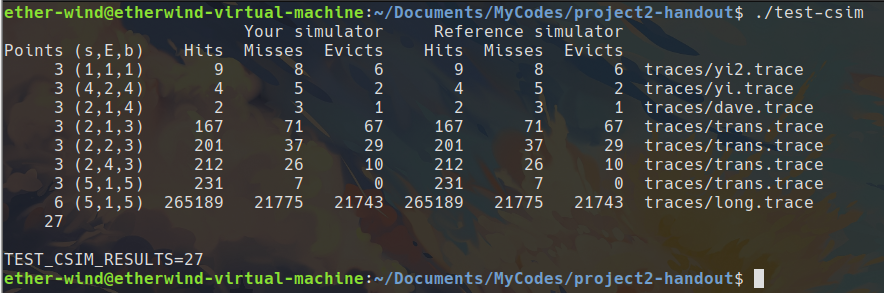
\includegraphics[width=0.7\linewidth]{csim.png}
    \caption{result of part A}\label{fig:1}
\end{figure}

\subsection{Part B}
 
\subsubsection{Analysis}

With twelve available variables, we can use at of them to store the elements in the matrix temperally when copy them into another matrix. This will reduce the number of evictions.

When $M = N = 32$, every eight raws of the matrix use different lines of the cache, and the capcity of the lines is also eight, so it its very natural to divide the matrix into sixteen $8 \times 8$ blocks and transpose the matrix in blocks. But there is a problem: if the block is on the diagonal, the original method to transpose the matrix will cause extra evictions. To solve this problem, we can store some elements at the same location in B, and then transfer it into the target location when the target location is loaded into the cache.

When $M = N = 64$, it will be more conplicated because in a $8 \times 8$ block, the first four lines use the same lines in the cache with the last four lines. If we still devide the matrix into $8 \times 8$ blocks, there sill be much more evictions. A simple idea is devide the matrix into $4 \times 4$ blocks, but it is also not very efficient. Here is another solution:. First devide the matrix into $8 \times 8$ large blocks, each large block is devided into four $4 \times 4$ small blocks. For each large blodk in A, if we want to transpose it into another large block in B, as what is shown in Figure \ref{fig:2}, do the following operations:

\begin{figure}[htbp]
    \centering
    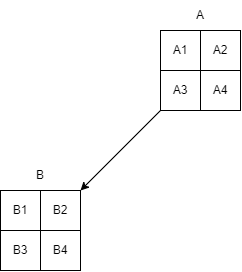
\includegraphics[width = 0.3\linewidth]{blocks.png}
    \caption{transpose A into B}\label{fig:2}
\end{figure}

\begin{itemize}
    \item $B_1 = A_1^T, B_2 = A_2^T$;
    \item $B_3 = B_2, B_2 = A_3^T$;
    \item $B_4 = A_4^T$.
\end{itemize}

It is important that when copy the elements, we should copy them in lines  to avoid evctions.

When $M = 61, N = 67$, it is much simpler than the second situation because there are not so many restrictions. The method in the first situation is OK in this case. The only difference is that there will additional incomplelte blocks to be deal with while it is very easy to realize.

\subsubsection{Code}

The code of \verb|csim.c| is shown in Code Listing \ref{cd:2}.

\begin{lstlisting}[language=c++, caption={trans.c}, label={cd:2}]
/* 
* trans.c - Matrix transpose B = A^T
*
* Each transpose function must have a prototype of the form:
* void trans(int M, int N, int A[N][M], int B[M][N]);
*
* A transpose function is evaluated by counting the number of misses
* on a 1KB direct mapped cache with a block size of 32 bytes.
*/ 
#include <stdio.h>
#include "cachelab.h"

int is_transpose(int M, int N, int A[N][M], int B[M][N]);

/* 
* transpose_submit - This is the solution transpose function that you
*     will be graded on for Part B of the assignment. Do not change
*     the description string "Transpose submission", as the driver
*     searches for that string to identify the transpose function to
*     be graded. 
*/
char transpose_submit_desc[] = "Transpose submission";
void transpose_submit(int M, int N, int A[N][M], int B[M][N])
{
    if (M == 32) {
        int i, j, x, y, tmp1, tmp2, tmp3, tmp4, tmp5, tmp6, tmp7, tmp8;
        for (i = 0; i < M; i += 8) {
            for (j = 0; j < N; j += 8)  {

                if (i != j) {
                    for (x = i; x < i + 8; ++x)
                    for (y = j; y < j + 8; ++y)
                        B[y][x] = A[x][y];
                }

                else {
                    tmp1 = A[i][j];
                    tmp2 = A[i][j + 1];
                    tmp3 = A[i][j + 2];
                    tmp4 = A[i][j + 3];
                    tmp5 = A[i][j + 4];
                    tmp6 = A[i][j + 5];
                    tmp7 = A[i][j + 6];
                    tmp8 = A[i][j + 7];

                    B[i][j] = tmp1;
                    B[i][j + 1] = tmp2;
                    B[i][j + 2] = tmp3;
                    B[i][j + 3] = tmp4;
                    B[i][j + 4] = tmp5;
                    B[i][j + 5] = tmp6;
                    B[i][j + 6] = tmp7;
                    B[i][j + 7] = tmp8;

                    tmp1 = A[i + 1][j];
                    tmp2 = A[i + 1][j + 1];
                    tmp3 = A[i + 1][j + 2];
                    tmp4 = A[i + 1][j + 3];
                    tmp5 = A[i + 1][j + 4];
                    tmp6 = A[i + 1][j + 5];
                    tmp7 = A[i + 1][j + 6];
                    tmp8 = A[i + 1][j + 7];

                    B[i + 1][j] = B[i][j + 1];
                    B[i][j + 1] = tmp1;
                    B[i + 1][j + 1] = tmp2;
                    B[i + 1][j + 2] = tmp3;
                    B[i + 1][j + 3] = tmp4;
                    B[i + 1][j + 4] = tmp5;
                    B[i + 1][j + 5] = tmp6;
                    B[i + 1][j + 6] = tmp7;
                    B[i + 1][j + 7] = tmp8;

                    tmp1 = A[i + 2][j];
                    tmp2 = A[i + 2][j + 1];
                    tmp3 = A[i + 2][j + 2];
                    tmp4 = A[i + 2][j + 3];
                    tmp5 = A[i + 2][j + 4];
                    tmp6 = A[i + 2][j + 5];
                    tmp7 = A[i + 2][j + 6];
                    tmp8 = A[i + 2][j + 7];

                    B[i + 2][j] = B[i][j + 2];
                    B[i + 2][j + 1] = B[i + 1][j + 2];
                    B[i][j + 2] = tmp1;
                    B[i + 1][j + 2] = tmp2;
                    B[i + 2][j + 2] = tmp3;
                    B[i + 2][j + 3] = tmp4;
                    B[i + 2][j + 4] = tmp5;
                    B[i + 2][j + 5] = tmp6;
                    B[i + 2][j + 6] = tmp7;
                    B[i + 2][j + 7] = tmp8;

                    tmp1 = A[i + 3][j];
                    tmp2 = A[i + 3][j + 1];
                    tmp3 = A[i + 3][j + 2];
                    tmp4 = A[i + 3][j + 3];
                    tmp5 = A[i + 3][j + 4];
                    tmp6 = A[i + 3][j + 5];
                    tmp7 = A[i + 3][j + 6];
                    tmp8 = A[i + 3][j + 7];

                    B[i + 3][j] = B[i][j + 3];
                    B[i + 3][j + 1] = B[i + 1][j + 3];
                    B[i + 3][j + 2] = B[i + 2][j + 3];
                    B[i][j + 3] = tmp1;
                    B[i + 1][j + 3] = tmp2;
                    B[i + 2][j + 3] = tmp3;
                    B[i + 3][j + 3] = tmp4;
                    B[i + 3][j + 4] = tmp5;
                    B[i + 3][j + 5] = tmp6;
                    B[i + 3][j + 6] = tmp7;
                    B[i + 3][j + 7] = tmp8;

                    tmp1 = A[i + 4][j];
                    tmp2 = A[i + 4][j + 1];
                    tmp3 = A[i + 4][j + 2];
                    tmp4 = A[i + 4][j + 3];
                    tmp5 = A[i + 4][j + 4];
                    tmp6 = A[i + 4][j + 5];
                    tmp7 = A[i + 4][j + 6];
                    tmp8 = A[i + 4][j + 7];

                    B[i + 4][j] = B[i][j + 4];
                    B[i + 4][j + 1] = B[i + 1][j + 4];
                    B[i + 4][j + 2] = B[i + 2][j + 4];
                    B[i + 4][j + 3] = B[i + 3][j + 4];
                    B[i][j + 4] = tmp1;
                    B[i + 1][j + 4] = tmp2;
                    B[i + 2][j + 4] = tmp3;
                    B[i + 3][j + 4] = tmp4;
                    B[i + 4][j + 4] = tmp5;
                    B[i + 4][j + 5] = tmp6;
                    B[i + 4][j + 6] = tmp7;
                    B[i + 4][j + 7] = tmp8;

                    tmp1 = A[i + 5][j];
                    tmp2 = A[i + 5][j + 1];
                    tmp3 = A[i + 5][j + 2];
                    tmp4 = A[i + 5][j + 3];
                    tmp5 = A[i + 5][j + 4];
                    tmp6 = A[i + 5][j + 5];
                    tmp7 = A[i + 5][j + 6];
                    tmp8 = A[i + 5][j + 7];

                    B[i + 5][j] = B[i][j + 5];
                    B[i + 5][j + 1] = B[i + 1][j + 5];
                    B[i + 5][j + 2] = B[i + 2][j + 5];
                    B[i + 5][j + 3] = B[i + 3][j + 5];
                    B[i + 5][j + 4] = B[i + 4][j + 5];
                    B[i][j + 5] = tmp1;
                    B[i + 1][j + 5] = tmp2;
                    B[i + 2][j + 5] = tmp3;
                    B[i + 3][j + 5] = tmp4;
                    B[i + 4][j + 5] = tmp5;
                    B[i + 5][j + 5] = tmp6;
                    B[i + 5][j + 6] = tmp7;
                    B[i + 5][j + 7] = tmp8;

                    tmp1 = A[i + 6][j];
                    tmp2 = A[i + 6][j + 1];
                    tmp3 = A[i + 6][j + 2];
                    tmp4 = A[i + 6][j + 3];
                    tmp5 = A[i + 6][j + 4];
                    tmp6 = A[i + 6][j + 5];
                    tmp7 = A[i + 6][j + 6];
                    tmp8 = A[i + 6][j + 7];

                    B[i + 6][j] = B[i][j + 6];
                    B[i + 6][j + 1] = B[i + 1][j + 6];
                    B[i + 6][j + 2] = B[i + 2][j + 6];
                    B[i + 6][j + 3] = B[i + 3][j + 6];
                    B[i + 6][j + 4] = B[i + 4][j + 6];
                    B[i + 6][j + 5] = B[i + 5][j + 6];
                    B[i][j + 6] = tmp1;
                    B[i + 1][j + 6] = tmp2;
                    B[i + 2][j + 6] = tmp3;
                    B[i + 3][j + 6] = tmp4;
                    B[i + 4][j + 6] = tmp5;
                    B[i + 5][j + 6] = tmp6;
                    B[i + 6][j + 6] = tmp7;
                    B[i + 6][j + 7] = tmp8;

                    tmp1 = A[i + 7][j];
                    tmp2 = A[i + 7][j + 1];
                    tmp3 = A[i + 7][j + 2];
                    tmp4 = A[i + 7][j + 3];
                    tmp5 = A[i + 7][j + 4];
                    tmp6 = A[i + 7][j + 5];
                    tmp7 = A[i + 7][j + 6];
                    tmp8 = A[i + 7][j + 7];

                    B[i + 7][j] = B[i][j + 7];
                    B[i + 7][j + 1] = B[i + 1][j + 7];
                    B[i + 7][j + 2] = B[i + 2][j + 7];
                    B[i + 7][j + 3] = B[i + 3][j + 7];
                    B[i + 7][j + 4] = B[i + 4][j + 7];
                    B[i + 7][j + 5] = B[i + 5][j + 7];
                    B[i + 7][j + 6] = B[i + 6][j + 7];
                    B[i][j + 7] = tmp1;
                    B[i + 1][j + 7] = tmp2;
                    B[i + 2][j + 7] = tmp3;
                    B[i + 3][j + 7] = tmp4;
                    B[i + 4][j + 7] = tmp5;
                    B[i + 5][j + 7] = tmp6;
                    B[i + 6][j + 7] = tmp7;
                    B[i + 7][j + 7] = tmp8;
                }
            }
        }
    }

    else if (M == 64) {
        int i, j, x, y, tmp1, tmp2, tmp3, tmp4, tmp5, tmp6, tmp7, tmp8;
        for (i = 0; i < M; i += 8) {
            for (j = 0; j < N; j += 8) {
                for (x = i; x < i + 4; ++x) {
                    tmp1 = A[x][j];
                    tmp2 = A[x][j + 1];
                    tmp3 = A[x][j + 2];
                    tmp4 = A[x][j + 3];
                    tmp5 = A[x][j + 4];
                    tmp6 = A[x][j + 5];
                    tmp7 = A[x][j + 6];
                    tmp8 = A[x][j + 7];

                    B[j][x] = tmp1;
                    B[j + 1][x] = tmp2;
                    B[j + 2][x] = tmp3;
                    B[j + 3][x] = tmp4;
                    B[j][x + 4] = tmp5;
                    B[j + 1][x + 4] = tmp6;
                    B[j + 2][x + 4] = tmp7;
                    B[j + 3][x + 4] = tmp8;
                }

                for (y = j; y < j + 4; ++y) {
                    tmp1 = A[i + 4][y];
                    tmp2 = A[i + 5][y];
                    tmp3 = A[i + 6][y];
                    tmp4 = A[i + 7][y];
                    tmp5 = B[y][i + 4];
                    tmp6 = B[y][i + 5];
                    tmp7 = B[y][i + 6];
                    tmp8 = B[y][i + 7];

                    B[y][i + 4] = tmp1;
                    B[y][i + 5] = tmp2;
                    B[y][i + 6] = tmp3;
                    B[y][i + 7] = tmp4;
                    B[y + 4][i] = tmp5;
                    B[y + 4][i + 1] = tmp6;
                    B[y + 4][i + 2] = tmp7;
                    B[y + 4][i + 3] = tmp8;
                }

                for (x = i + 4; x < i + 8; ++x) {
                    tmp1 = A[x][j + 4];
                    tmp2 = A[x][j + 5];
                    tmp3 = A[x][j + 6];
                    tmp4 = A[x][j + 7];

                    B[j + 4][x] = tmp1;
                    B[j + 5][x] = tmp2;
                    B[j + 6][x] = tmp3;
                    B[j + 7][x] = tmp4;
                }
            }
        }
    }

    else if (M == 61) {
        int i, j, tmp1, tmp2, tmp3, tmp4, tmp5, tmp6, tmp7, tmp8;
        int n = N / 8 * 8;
        int m = M / 8 * 8;
        for (j = 0; j < m; j += 8) {
            for (i = 0; i < n; ++i) {
                tmp1 = A[i][j];
                tmp2 = A[i][j+1];
                tmp3 = A[i][j+2];
                tmp4 = A[i][j+3];
                tmp5 = A[i][j+4];
                tmp6 = A[i][j+5];
                tmp7 = A[i][j+6];
                tmp8 = A[i][j+7];
                
                B[j][i] = tmp1;
                B[j+1][i] = tmp2;
                B[j+2][i] = tmp3;
                B[j+3][i] = tmp4;
                B[j+4][i] = tmp5;
                B[j+5][i] = tmp6;
                B[j+6][i] = tmp7;
                B[j+7][i] = tmp8;
            }
        }
        for (i = n; i < N; ++i) {
            for (j = m; j < M; ++j) {
                tmp1 = A[i][j];
                B[j][i] = tmp1;
            }
        }
        for (i = 0; i < N; ++i) {
            for (j = m; j < M; ++j) {
                tmp1 = A[i][j];
                B[j][i] = tmp1;
            }
        }
        for (i = n; i < N; ++i) {
            for (j = 0; j < M; ++j) {
                tmp1 = A[i][j];
                B[j][i] = tmp1;
            }
        }
    }
}

/* 
* You can define additional transpose functions below. We've defined
* a simple one below to help you get started. 
*/ 

/* 
* trans - A simple baseline transpose function, not optimized for the cache.
*/
char trans_desc[] = "Simple row-wise scan transpose";
void trans(int M, int N, int A[N][M], int B[M][N])
{
    int i, j, tmp;

    for (i = 0; i < N; i++) {
        for (j = 0; j < M; j++) {
            tmp = A[i][j];
            B[j][i] = tmp;
        }
    }    

}

/*
* registerFunctions - This function registers your transpose
*     functions with the driver.  At runtime, the driver will
*     evaluate each of the registered functions and summarize their
*     performance. This is a handy way to experiment with different
*     transpose strategies.
*/
void registerFunctions()
{
    /* Register your solution function */
    registerTransFunction(transpose_submit, transpose_submit_desc); 

    /* Register any additional transpose functions */
    registerTransFunction(trans, trans_desc); 

}

/* 
* is_transpose - This helper function checks if B is the transpose of
*     A. You can check the correctness of your transpose by calling
*     it before returning from the transpose function.
*/
int is_transpose(int M, int N, int A[N][M], int B[M][N])
{
    int i, j;

    for (i = 0; i < N; i++) {
        for (j = 0; j < M; ++j) {
            if (A[i][j] != B[j][i]) {
            return 0;
            }
        }
    }
    return 1;
}
    
\end{lstlisting}

\subsubsection{Evaluation}

the detailed results of part B are shown in Figure \ref{fig:3}. The brief results are shown in Figure \ref{fig:4}, which is implemented by \verb|driver.py|.

\begin{figure}[htbp]
    \centering
    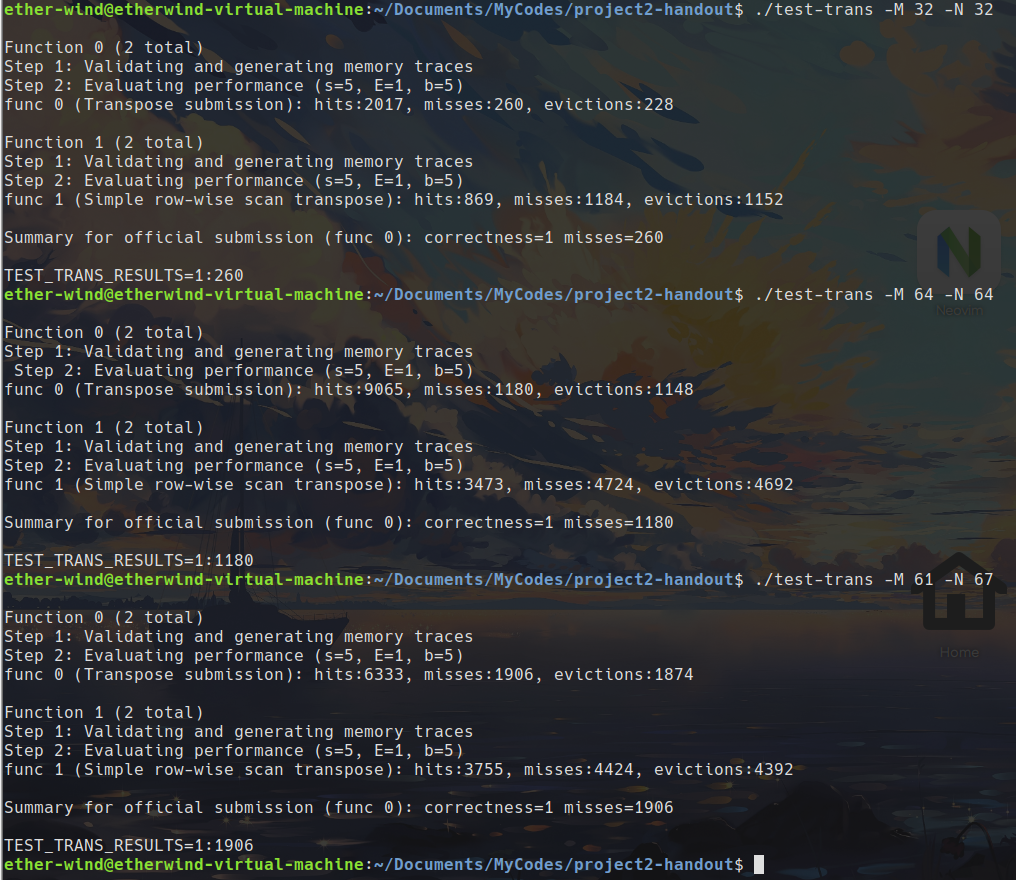
\includegraphics[width = 0.7\linewidth]{trans-detail.png}
    \caption{detailed results}\label{fig:3}
\end{figure}

\begin{figure}[htbp]
    \centering
    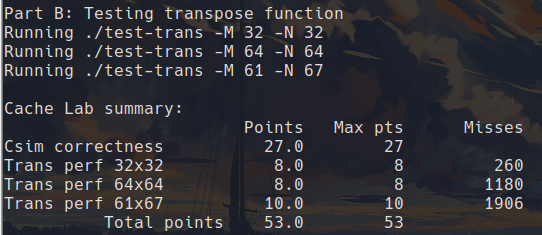
\includegraphics[width = 0.7\linewidth]{trans-total.png}
    \caption{brief results}\label{fig:4}
\end{figure}

As what we can see in the figures, the results of the three tests are all correct and achieve full marks.

\section{Conclusion}

\subsection{Problems}

The biggest problem is that how to reduce evictions in part B, especially when $M = N = 64$. I have tried to use $8 \times 8$ and $4 \times 4$ blocks but the result is not satisfying. And finally I successfully combine the two method, which I have mentioned above. 

\subsection{Achievements}

In my sulotion, I take full use of the twelve variables, and use block technique to improvement the performance. I also design different algorithms for different inputs.

To increase the coding readability, I seperate different sections with empty lines, add necessary commentions and keep the code as neat as possible.

In this project, I have a deeper understanding of caching and learn about block technique. I feel that I benefit from this project a lot.

%----------------------------------------------------------------------------------------


\end{document}